\documentclass{beamer}
\mode<presentation>

\usetheme{Madrid}

\usepackage{lipsum}

\usepackage{listings}
\usepackage{caption}

\lstset{
    language=Python,
    basicstyle=\small\ttfamily,
    numbers=left,
    numbersep=5pt,
    xleftmargin=20pt,
    frame=tb,
    framexleftmargin=20pt
}

\renewcommand*\thelstnumber{\arabic{lstnumber}:}

\DeclareCaptionFormat{mylst}{\hrule#1#2#3}
\captionsetup[lstlisting]{format=mylst,labelfont=bf,singlelinecheck=off,labelsep=space}


\usepackage{graphicx}
\usepackage{float}
\graphicspath{{Images}}



\title{Licen\c t\u a informatic\u a}
\subtitle{Problema Reginelor}
\author{A. Student\inst{1} Guțic Constantin-Gabriel\inst{2} \\
    A. Student\inst{1} Iacob Iustina\inst{2}
}
\institute{
    \inst{1}
    Facultatea de Matematic\u a \\
    Specializarea Matematic\u a - Informatic\u a
    \and
    \inst{2}
    Universitatea "Al. I. Cuza" Ia\c si\\
    Facultatea de Matematic\u a
}
\date{Iulie 2022}


\begin{document}
    
\frame{\titlepage}

\begin{frame}{Cuprins}
    \tableofcontents[currentsection]
\end{frame}

\begin{frame}{Problema reginelor}
    \begin{block}{Enun\c t}
        Dându-se o tablă de 
        şah de dimensiune nxn (\(n > 1\)) să se aranjeze 
        pe ea n regine fără ca ele să se atace. 
        Reamintim că o regină atacă linia, coloana 
        şi cele 2 diagonale pe care se află. În 
        figura de mai jos celulele colorate mai 
        închis sunt atacate de regina poziţionată \^ in caseta (0, 0).
    \end{block}
    \begin{figure}
        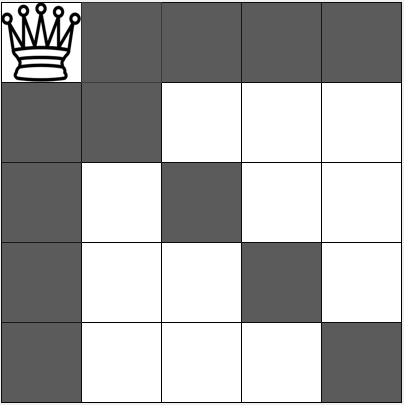
\includegraphics[width=0.3\textwidth]{1.png}
    \end{figure}
\end{frame}

\begin{frame}[fragile]{Crearea ferestrei \c si a tabelului}
    \begin{block}{Descriere}
        \lipsum[1][1-3]
    \end{block}

    \begin{lstlisting}[caption={Slider creation}]
window = Window("Queen", 800, 600)

table = Table(window, 5, center=Point(400, 300))
    \end{lstlisting}
\end{frame}

\begin{frame}[fragile]{Punctul de pornire al algoritmului}

\begin{lstlisting}[caption={Start Function}]
def start():
    slider_rows.set_visible(False)
    start_button.set_visible(False)
    w = table.squares[0][0].width
    for i in range(table.rows):
        queens.append({
        'col': None,
        'image': Image(window, width=w, height=w, 
                        path="../images/queen.png"),
        })
        queens[i]['image'].set_visible(False)

    backtracking_thread = threading.Thread(
        target=backtracking_init)
    backtracking_thread.start()
\end{lstlisting}
    
\end{frame}

\begin{frame}{Algoritmul}
    \begin{block}{Explica\c tie 1}
        \lipsum[1][1]
    \end{block}

    \begin{block}{Explica\c tie 2}
        \lipsum[1][1-2]
    \end{block}

    \begin{block}{Explica\c tie 3}
        \lipsum[2][1-3]
    \end{block}
\end{frame}

\begin{frame}[fragile]{Algoritmul}
    \begin{block}{Explica\c tie}
        \lipsum[1][1-2]
    \end{block}

    \begin{lstlisting}{Code}
def back(k):
    for i in range(table.rows):
        global is_running
        if not is_running:
            return False
        queens[k]['col'] = i
        queens[k]['image'].center = 
                table.squares[k][i].center
        queens[k]['image'].set_visible(True)

    \end{lstlisting}
\end{frame}

\begin{frame}[fragile]{Algoritmul}
    \begin{lstlisting}
        pause()
        if valid(k):
            if solution(k):
                show_solution()
            else:
                back(k + 1)
    queens[k]['image'].set_visible(False)
    pause()
    \end{lstlisting}

    \begin{block}{Precizare}
        \lipsum[1][3-5]
    \end{block}
\end{frame}

\end{document}